\chapter{Results}
\section{Potential fields}
The MATLAB simulations proved the validity of the potential field control algorithm, as an n-number of robot convoys successfully followed the leader's trajectory, while maintaining a constant distance from each other. In addition, the smoothing control algorithm was also proven during simulation, as the following robots were able to follow a smoother trajectory to the goal, resulting in less radical turns and directional adjustments. In a more realistic situation, if a following robots leader disappears (i.e. breaks down) the follower becomes the leader and reaches its goal.

\section{Dynamics}
Running each of the dynamic models (quarter car, half car, full car,) produced a set of graphs detailing the system response. These showed the system traversing several terrain types, but for the clarity of this report, only the system traversing a 2cm bump directly was included (more thorough results can be found in appendix \ref{a:dynamics_response}). This is one of the worse-case scenarios the system would have to deal with, and produces the clearest graphs. Once the simulation is run, the car is given 3 seconds or flat terrain for the system to settle from its 0-configuration before it hits the 2cm bump. In the first 3 seconds, the system can be clearly seen undergoing a damped oscillation to its equilibrium position. The half car and full car models also show the roll and pitch of the system respectively. For this simulation, the geometry was defined such that there would be no lateral or horizontal displacement. At the 3 second mark, the system can be seen traversing the bump. This is most pronounced in the quarter car model, as the shock and damper system absorb the majority of the body displacement in the half car and full car models. The effect of the bump can still be seen on the wheels though. The bump can also be seen effecting a pitch in the full car model. As the front wheels hit the bump, the car pitches upwards until the back wheels hit the bump causing a matched downward pitch. This induces some oscillations which become damped quickly.

Running concurrently with the dynamics are the inverse dynamics. These are calculated from the point of view of a system following the leader. The inverse dynamic model is able to correctly predict the sag of the system from its 0-configuration within 1\% error. For most of the terrain we generated, the inverse dynamics were able to correctly predict the response of the system within 2\%-5\% error. These large bumps are the most extreme case we were able to find. They exhibit up to 10\% instantaneous error; however they drop back to a baseline 1\% error within 0.2 seconds. This error is a result of the naive approach taken with calculating the wheel states using the last time step. If the states were filtered, the estimates are even closer. However, there was not time to create a rigorous filter for this purpose.

\begin{figure}[t]
	\centering
	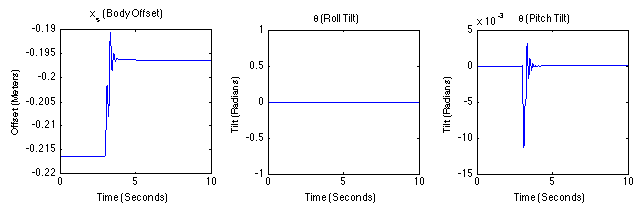
\includegraphics[width=1.0\textwidth]{figures/results_2cm_body.png}
	\caption{The body response of a car traversing a 2cm bump head on.}
	\label{fig:fullcar_2cm_body}
\end{figure}

\begin{figure}[t]
	\centering
	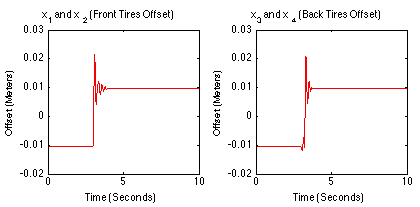
\includegraphics[width=0.65\textwidth]{figures/results_2cm_wheel.png}
	\caption{The wheel response of a car traversing a 2cm bump head on.}
	\label{fig:fullcar_2cm_wheel}
\end{figure}

\begin{figure}[t]
	\centering
	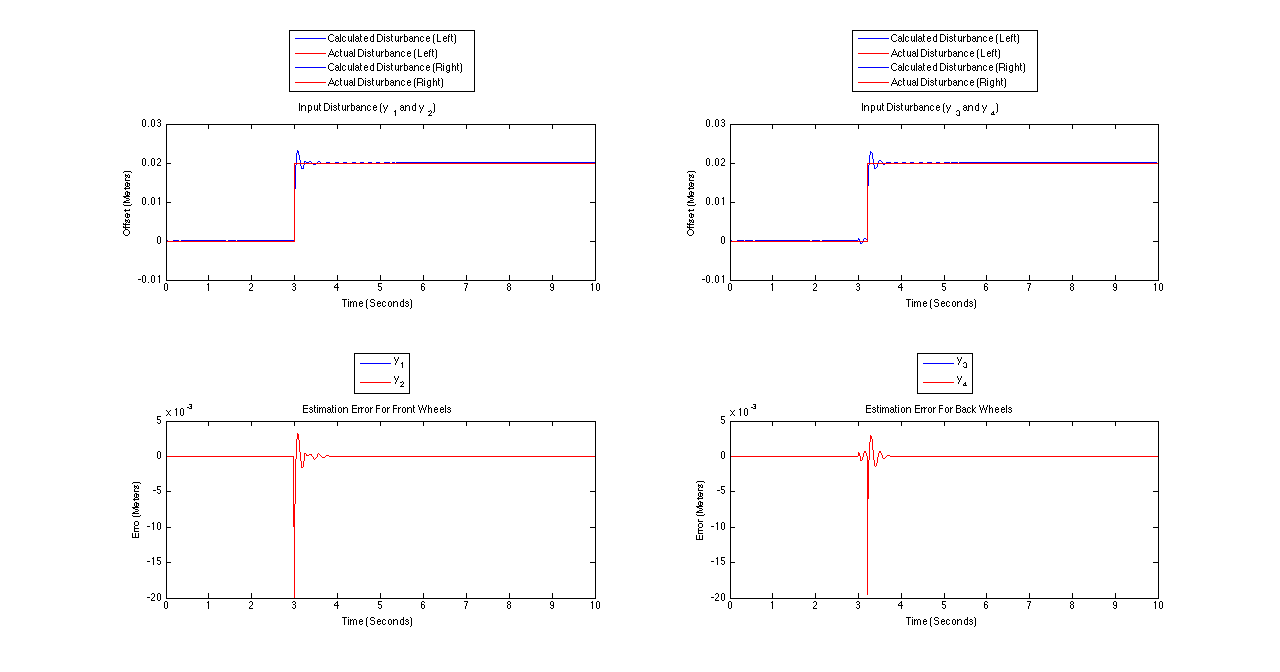
\includegraphics[width=1.0\textwidth]{figures/fullcar_2cm_straight_inverse.png}
	\caption{The estimation of a car traversing a 2cm bump head on.}
	\label{fig:fullcar_2cm}
\end{figure}

